% !TEX program = pdflatex
\documentclass[11pt,a4paper]{article}

\usepackage[margin=2.05cm]{geometry}
\usepackage[T1]{fontenc}
\usepackage[utf8]{inputenc}
\usepackage{lmodern}
\usepackage{microtype}
\usepackage{amsmath,amssymb,amsthm}
\usepackage{booktabs}
\usepackage{tabularx}
\usepackage{array}
\usepackage{xcolor}
\usepackage{graphicx}
\usepackage{float}
\usepackage{caption}
\usepackage{subcaption}
\usepackage{tikz}
\usetikzlibrary{arrows.meta,positioning,fit,calc,shapes.geometric}
\usepackage[colorlinks,citecolor=blue!70!black,linkcolor=blue!70!black,urlcolor=blue!50!black]{hyperref}
\usepackage[capitalise,noabbrev]{cleveref}

\newcolumntype{Y}{>{\raggedright\arraybackslash}X}
\setlength{\emergencystretch}{3em}

\newtheorem{theorem}{Theorem}[section]
\newtheorem{lemma}[theorem]{Lemma}
\newtheorem{claim}[theorem]{Claim}
\theoremstyle{definition}
\newtheorem{definition}[theorem]{Definition}
\newtheorem{remark}[theorem]{Remark}

\newcommand{\Aura}{\textsc{Aura}}
\newcommand{\MLS}{\textsf{MLS}}
\newcommand{\TreeKEM}{\textsf{TreeKEM}}
\newcommand{\Shield}{\textsf{Shield}}
\newcommand{\HKDF}{\textsf{HKDF}}
\newcommand{\HMAC}{\textsf{HMAC}}
\newcommand{\SHA}{\textsf{SHA-256}}
\newcommand{\AEAD}{\textsf{AES-256-GCM-SIV}}
\newcommand{\BLAKE}{\textsf{BLAKE2b}}
\newcommand{\EdDSA}{\textsf{Ed25519}}
\renewcommand{\DH}{\textsf{X25519}}
\newcommand{\KEM}{\textsf{ML-KEM-768}}
\newcommand{\Enc}{\textsf{Enc}}
\newcommand{\Dec}{\textsf{Dec}}
\newcommand{\KeyGen}{\textsf{KeyGen}}
\newcommand{\Encaps}{\textsf{Encaps}}
\newcommand{\Decaps}{\textsf{Decaps}}
\newcommand{\concat}{\,\|\,}
\newcommand{\gid}{\mathit{gid}}
\newcommand{\epoch}{\mathit{epoch}}
\newcommand{\gch}{\mathit{gch}}
\newcommand{\initsec}{\mathit{init}}
\newcommand{\commitsec}{\mathit{commit}}
\newcommand{\epochsec}{\mathit{epochSecret}}
\newcommand{\policy}{\mathit{policy}}
\newcommand{\treehash}{\mathit{treeHash}}

\title{\textbf{Aura Group: Policy-Bound Hybrid TreeKEM for Post-Quantum Group Messaging}}

\author{%
  Oleksandr Melnychenko\\
  \texttt{oleksandr@aura.io}
}

\date{\today}

\begin{document}
\maketitle

\begin{abstract}
\Aura{} Group is a group-messaging construction that extends the two-party
\Aura{} design discipline to an MLS-inspired setting. Its group state is
advanced by \TreeKEM{}-style commits whose update path carries both \DH{}
and \KEM{} public keys. Path secrets are encrypted to co-path resolutions with
a hybrid \DH{}+\KEM{} wrapping key, and every accepted commit derives a new
epoch secret from the previous init secret, the fresh commit secret, and a
context hash that includes the group identifier, epoch number, tree hash, and
serialized security policy.

The central contribution is not the isolated use of TreeKEM or ML-KEM. It is
the combination of hybrid update paths with a policy-bound epoch context:
security policy is treated as cryptographic input, not as application metadata.
The \Shield{} profile fixes a stricter policy for high-risk groups by enabling
an enhanced key schedule, requiring message franking, blocking external joins,
and bounding sender-key lifetime and skipped-key storage. The message layer
then uses per-member sender chains, encrypted sender data, replay windows,
sealed content, expiring content, and franking commitments without giving the
relay access to group plaintext or group secrets.

This paper gives the construction, implementation evidence, and a scoped
security argument. The claims are intentionally narrower than a full MLS
proof: the implementation supports membership-change forward secrecy,
epoch-level post-compromise recovery through hybrid update paths, policy
consensus through confirmation MACs, and message-level replay and franking
checks. A complete symbolic or game-based proof for concurrent group sessions
remains future work.
\end{abstract}

\smallskip
\noindent\textbf{Keywords:} group messaging, TreeKEM, MLS, post-quantum cryptography, ML-KEM, sender keys, message franking, replay protection.

\tableofcontents
\newpage

\section{Introduction}

End-to-end encrypted group messaging has a different shape from a two-party
ratchet. A two-party channel can update state along a single pairwise
timeline. A group channel must update membership, distribute fresh secrets to
the current roster, exclude removed members, preserve sender authentication,
and keep application messages inexpensive between membership changes.
\MLS{} standardizes this problem space with TreeKEM-based epoch transitions
and a group key schedule~\cite{rfc9420}. The post-quantum setting adds a
further constraint: a group update that only refreshes classical DH material
does not address recorded traffic against a future cryptographically relevant
quantum computer.

The companion \Aura{} foundation paper studies the two-party handshake and
ratchet boundary. This paper is deliberately separate. The group construction
reuses the same primitive discipline--\DH{}, \KEM{}, \HKDF{}, and misuse-
resistant AEAD--but its security statements concern group state, epoch commits,
sender chains, and relay-visible envelopes. The two-party theorems do not
automatically imply group security; group messaging needs its own tree-state
and concurrency analysis. In this paper, \emph{artifact} means the
implementation, tests, benchmarks, and design notes that accompany the
construction.

\paragraph{Scientific novelty.}
The scientific novelty of \Aura{} Group is the design and implementation
validation of a policy-bound hybrid TreeKEM construction for group messaging.
The main points are:

\begin{enumerate}
  \item \textbf{Hybrid post-quantum update path.} Each epoch-changing update
  refreshes TreeKEM path material with \DH{} and \KEM{} keys, rather than
  limiting post-quantum material to group creation.

  \item \textbf{Policy-bound group context.} The group context hash includes
  the serialized security policy. A policy disagreement changes epoch keys and
  confirmation MACs, so policy becomes part of cryptographic consensus.

  \item \textbf{Shielded epoch profile.} \Shield{} is specified as a
  cryptographic policy profile: enhanced subkey derivation, mandatory
  franking, external-join blocking, bounded skipped keys, and bounded
  sender-key lifetime.

  \item \textbf{Efficient message layer inside an epoch.} Per-member sender
  chains provide low-cost application messages between TreeKEM commits, while
  encrypted sender data and replay windows preserve epoch binding and duplicate
  rejection.

  \item \textbf{Accountable encrypted semantics.} Franking, sealed content,
  and disappearing messages are integrated as message semantics over the group
  key schedule without exposing plaintext to the relay.
\end{enumerate}

\section{Threat Model and Scope}

The adversary controls the network, reorders and replays messages, corrupts
old serialized state, tampers with commits and application ciphertexts, and may
learn secrets of removed members. The relay is not trusted with plaintext or
group secrets. It may validate structure and route messages, but authoritative
membership and epoch state are client-side decisions.

The paper studies a single-device group model. Identity authentication uses
Ed25519 signatures over key packages and commits. This is classical
authentication; a transition to post-quantum signatures is orthogonal to the
TreeKEM and policy-binding mechanisms. The current evidence is implementation
evidence plus a protocol argument. A full theorem for asynchronous concurrent
groups, including delivery schedules and all interleavings of Add, Remove,
Update, PSK, and ReInit proposals, is not claimed here.

\begin{table}[H]
\centering
\caption{Claim boundary for the group paper.}\label{tab:scope}
\small
\begin{tabularx}{\textwidth}{@{}p{0.29\textwidth}YY@{}}
\toprule
Topic & Claimed in this paper & Not claimed in this paper \\
\midrule
Epoch secrecy & Fresh epoch keys after accepted hybrid TreeKEM commits, subject to at least one unbroken component and honest erasure. & A full universal-composability proof for all concurrent group schedules. \\
Post-compromise recovery & Recovery at epoch boundaries when an honest update path introduces fresh \DH{} and \KEM{} material after compromise. & Recovery without a later honest epoch update. \\
Policy enforcement & Policy bytes are hashed into the group context and affect epoch keys and confirmation MACs. & Server-side policy authority or mutable policy negotiation. \\
Relay role & Relay-blind structural validation and routing. & Relay knowledge of plaintext, group secrets, or authoritative membership state. \\
Application semantics & Franking, sealed content, and expiration are enforced at message processing boundaries. & Legal moderation semantics beyond cryptographic verification of a disclosed message. \\
\bottomrule
\end{tabularx}
\end{table}

\section{Construction Overview}

\Aura{} Group has three layers. The epoch layer maintains a ratchet tree and
advances it with commits. The key-schedule layer derives epoch secrets,
metadata keys, welcome keys, confirmation keys, and sender-key bases. The
message layer encrypts application payloads under per-sender chains while
encrypting sender metadata under the epoch metadata key.

The tree is left-balanced and stores both \DH{} and \KEM{} public material at
leaves and internal nodes. A member's key package binds identity \EdDSA{},
identity \DH{}, identity \KEM{}, leaf \DH{}, leaf \KEM{}, and credential bytes
under an \EdDSA{} signature. This separates long-term identity from epoch
update material while giving recipients a signed object for membership
admission.

\begin{figure}[H]
\centering
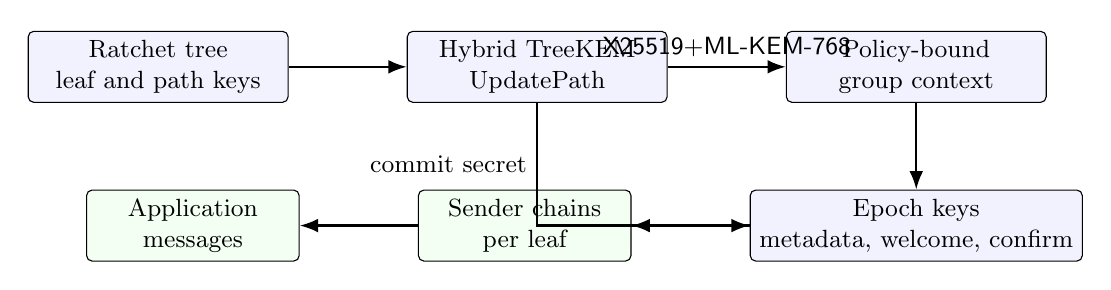
\begin{tikzpicture}[
  font=\small,
  node distance=1.1cm and 1.5cm,
  block/.style={draw,rounded corners=2pt,align=center,minimum width=3.3cm,minimum height=0.85cm,fill=blue!5},
  smallblock/.style={draw,rounded corners=2pt,align=center,minimum width=2.7cm,minimum height=0.78cm,fill=green!5},
  arrow/.style={-Latex,thick}
]
\node[block] (tree) {Ratchet tree\\leaf and path keys};
\node[block,right=of tree] (commit) {Hybrid TreeKEM\\UpdatePath};
\node[block,right=of commit] (ctx) {Policy-bound\\group context};
\node[block,below=of ctx] (epoch) {Epoch keys\\metadata, welcome, confirm};
\node[smallblock,left=of epoch] (sender) {Sender chains\\per leaf};
\node[smallblock,left=of sender] (msg) {Application\\messages};

\draw[arrow] (tree) -- (commit);
\draw[arrow] (commit) -- node[above]{\DH{}+\KEM{}} (ctx);
\draw[arrow] (ctx) -- (epoch);
\draw[arrow] (epoch) -- (sender);
\draw[arrow] (sender) -- (msg);
\draw[arrow] (commit.south) |- node[pos=0.25,left]{commit secret} (epoch.west);
\end{tikzpicture}
\caption{Epoch transition and message-key flow. A commit updates the tree,
derives a policy-bound context, and refreshes sender chains for the new epoch.}
\label{fig:epoch-flow}
\end{figure}

\subsection{Key Packages and Welcome}

Adding a member produces a signed key package, a commit, and a Welcome message.
The Welcome encrypts the joiner secret for the added member and carries enough
public group information for the recipient to reconstruct the tree, verify the
tree hash, parse the serialized policy, derive epoch keys, and check the
confirmation MAC. The design therefore keeps admission state explicit: a
member joins after decrypting Welcome and accepting the resulting epoch state,
not because the relay appended an identity to a roster.

\begin{table}[H]
\centering
\caption{Group-state objects and their role.}\label{tab:objects}
\small
\begin{tabularx}{\textwidth}{@{}p{0.24\textwidth}YY@{}}
\toprule
Object & Contents & Role in the construction \\
\midrule
Key package & Identity keys, leaf update keys, credential, signature. & Authenticated input for adding a member to the tree. \\
UpdatePath & Leaf public keys, path node public keys, encrypted path secrets, parent hashes. & Refreshes epoch tree material for current members. \\
Group context hash & Group identifier, epoch, tree hash, serialized policy. & Binds key derivation to tree state and security policy. \\
Welcome & Encrypted joiner secret and public group information. & Allows a newly added member to reconstruct and verify epoch state. \\
Application message & Encrypted sender data, encrypted payload, nonces, signature, optional franking tag. & Carries in-epoch traffic under sender-chain keys. \\
\bottomrule
\end{tabularx}
\end{table}

\subsection{Hybrid Update Path}

For a commit at epoch $e$, the committer samples a fresh path secret and
derives node secrets along its direct path. Each updated node receives a fresh
\DH{} keypair and a fresh \KEM{} keypair. For every recipient resolution node,
the path secret is wrapped under a hybrid key:
\begin{align*}
  x_{\mathsf{eph}}, X_{\mathsf{eph}} &\gets \DH.\KeyGen(), \\
  z_{\DH} &= \DH(x_{\mathsf{eph}}, X_R), \\
  (c_{\KEM}, z_{\KEM}) &\gets \KEM.\Encaps(pk_R), \\
  s_{\mathsf{path}} &= \textsf{``Aura-Group-Hybrid''}\concat z_{\DH}, \\
  i_{\mathsf{path}} &= \textsf{``PathSecret''}, \\
  k_{\mathsf{path}} &= \HKDF(z_{\KEM};s_{\mathsf{path}},i_{\mathsf{path}}), \\
  C_{\mathsf{path}} &= \AEAD.\Enc(k_{\mathsf{path}},n,\mathit{pathSecret},\mathit{nodeIndex}).
\end{align*}
The corresponding recipient decapsulates $c_{\KEM}$, computes the matching
\DH{} value, reconstructs $k_{\mathsf{path}}$, and decrypts the path secret.
The node index is associated data, so a wrapped path secret cannot be moved to
another tree position without detection. Parent hashes are verified along the
updated path so that an adversary cannot splice a valid node into an
inconsistent tree transcript.

\subsection{Policy-Bound Epoch Context}

The epoch context is defined with length prefixes for variable-size fields:
\begin{equation}
  \gch_e =
  \SHA\!\left(
    \ell(\gid)\concat \gid \concat
    e \concat
    \ell(\treehash_e)\concat \treehash_e \concat
    \ell(\policy)\concat \policy
  \right).
  \label{eq:gch}
\end{equation}
The length prefixes remove concatenation ambiguity. More importantly, the
serialized policy is inside the hash. If two members disagree on whether
\Shield{} is enabled, or on the sender-key limits, they compute different
$\gch_e$, different epoch keys, and different confirmation MACs.

The epoch keys are then derived as:
\begin{align}
  j_e &= \HKDF\text{-}\mathrm{Extract}(\initsec_{e-1}, \commitsec_e),\\
  \epochsec_e &=
  \HKDF\text{-}\mathrm{Expand}(j_e,\;
    \textsf{``Aura-Group-EpochSecret''}\concat \gch_e),\\
  (k^{\mathsf{meta}}_e,k^{\mathsf{welcome}}_e,k^{\mathsf{confirm}}_e,\initsec_e)
  &\gets \mathrm{Subkeys}(\epochsec_e).
  \label{eq:epoch-keys}
\end{align}
The confirmation MAC is:
\begin{equation}
  \tau_e = \HMAC(k^{\mathsf{confirm}}_e,\gch_e).
  \label{eq:confirmation}
\end{equation}
Thus the confirmation step checks tree state and policy state together.

\subsection{Shield Mode}

\Shield{} is a fixed stricter policy profile. Its default values are
$1000$ messages per epoch, $4$ skipped sender keys per sender, external joins
blocked, enhanced key schedule enabled, and mandatory franking enabled.
Enhanced subkey derivation uses two HKDF-Expand passes with distinct labels:
\begin{align}
  t &= \HKDF\text{-}\mathrm{Expand}(\epochsec_e,\mathit{info}\concat\textsf{pass1}),\\
  k &= \HKDF\text{-}\mathrm{Expand}(t,\mathit{info}\concat\textsf{pass2}).
\end{align}
The goal is not to replace the security assumption of HKDF, but to make the
\Shield{} profile an explicit, checkable domain-separated key schedule rather
than a set of advisory application flags.

\begin{figure}[H]
\centering
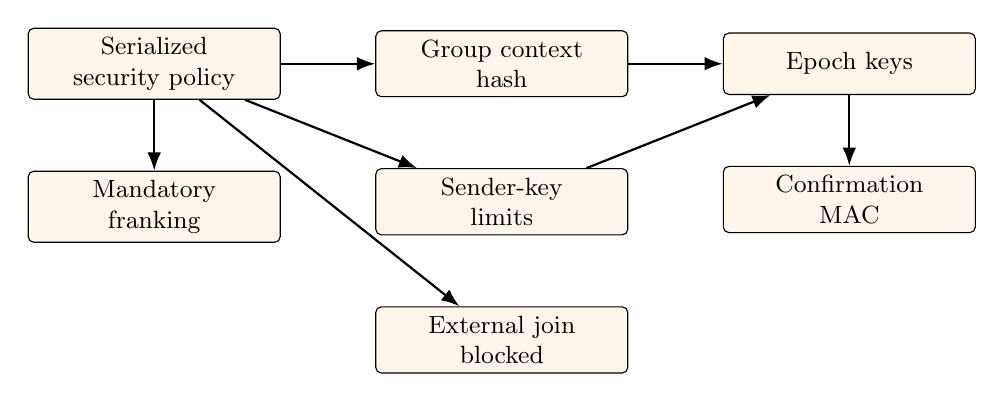
\begin{tikzpicture}[
  font=\small,
  box/.style={draw,rounded corners=2pt,align=center,minimum width=3.2cm,minimum height=0.78cm,fill=orange!8},
  arrow/.style={-Latex,thick},
  node distance=0.9cm and 1.2cm
]
\node[box] (policy) {Serialized\\security policy};
\node[box,right=of policy] (hash) {Group context\\hash};
\node[box,right=of hash] (keys) {Epoch keys};
\node[box,below=of keys] (confirm) {Confirmation\\MAC};
\node[box,below=of hash] (sender) {Sender-key\\limits};
\node[box,below=of policy] (frank) {Mandatory\\franking};
\node[box,below=of sender] (join) {External join\\blocked};

\draw[arrow] (policy) -- (hash);
\draw[arrow] (hash) -- (keys);
\draw[arrow] (keys) -- (confirm);
\draw[arrow] (policy) -- (frank);
\draw[arrow] (policy) -- (sender);
\draw[arrow] (policy) -- (join);
\draw[arrow] (sender) -- (keys);
\end{tikzpicture}
\caption{\Shield{} as a cryptographic policy profile. Policy bytes affect
epoch derivation and also drive local message-processing limits.}
\label{fig:shield}
\end{figure}

\section{Message Layer}

TreeKEM commits are comparatively expensive and are used for epoch changes.
Inside one epoch, application messages use sender chains. For sender leaf $i$
and generation $g$:
\begin{align}
  mk_{i,g} &= \HKDF\text{-}\mathrm{Expand}(ck_{i,g},\textsf{``Aura-Group-Msg''}),\\
  ck'_{i,g+1} &= \HKDF\text{-}\mathrm{Expand}(ck_{i,g},\textsf{``Aura-Group-Chain''}),\\
  ck_{i,g+1} &=
  \begin{cases}
    ck'_{i,g+1}, & \text{default policy},\\
    \BLAKE_{\textsf{Aura-B2Chain}}(ck'_{i,g+1}), & \Shield{}.
  \end{cases}
\end{align}
The payload is padded and encrypted under $mk_{i,g}$. Sender metadata
$(i,g,\mathit{reuseGuard})$ is encrypted under the epoch metadata key
$k^{\mathsf{meta}}_e$. The message signature covers the group identifier,
epoch, encrypted sender data, encrypted payload, nonces, and franking tag.

\subsection{Replay Rejection}

Each sender has a replay window with a high-water generation and a bitmap.
A duplicate generation inside the window is rejected. A generation too far
behind the window is also rejected. The skipped-key cache is bounded per
sender and globally; \Shield{} tightens the per-sender bound.

\subsection{Franking, Sealed Content, and Expiration}

For a frankable message the sender samples a franking key $fk$ and publishes:
\begin{equation}
  \mathit{tag} = \HMAC(fk,\mathit{content}\concat\mathit{sealedContent}).
  \label{eq:franking}
\end{equation}
The tag is visible in the application message, while $fk$ is inside the
end-to-end encrypted payload. A recipient who reports a message can disclose
$(fk,\mathit{content})$ for that message only. The relay cannot verify or read
unreported messages because it does not know $fk$.

Sealed content places an encrypted inner payload behind a visible hint. The
seal key is derived from the message key, and the recipient obtains it only
after group decryption. Disappearing messages carry a send timestamp and TTL;
decryption rejects expired messages and timestamps too far in the future.

\begin{figure}[H]
\centering
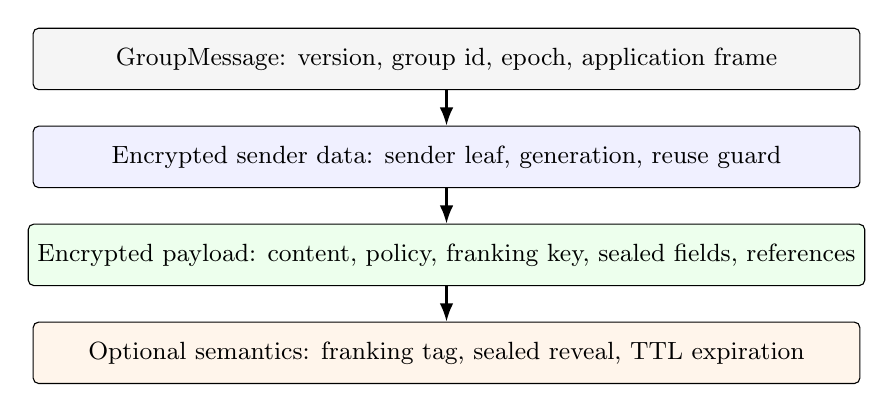
\begin{tikzpicture}[
  font=\small,
  layer/.style={draw,rounded corners=2pt,align=center,minimum width=10.5cm,minimum height=0.78cm},
  arrow/.style={-Latex,thick}
]
\node[layer,fill=gray!8] (wire) {GroupMessage: version, group id, epoch, application frame};
\node[layer,below=0.45cm of wire,fill=blue!6] (sender) {Encrypted sender data: sender leaf, generation, reuse guard};
\node[layer,below=0.45cm of sender,fill=green!7] (payload) {Encrypted payload: content, policy, franking key, sealed fields, references};
\node[layer,below=0.45cm of payload,fill=orange!8] (sem) {Optional semantics: franking tag, sealed reveal, TTL expiration};
\draw[arrow] (wire) -- (sender);
\draw[arrow] (sender) -- (payload);
\draw[arrow] (payload) -- (sem);
\end{tikzpicture}
\caption{Application-message envelope. Sender data is hidden from passive
observers under the epoch metadata key, while the payload uses the sender-chain
message key.}
\label{fig:message-envelope}
\end{figure}

\section{External Join and Relay Model}

External join is supported only when policy permits it. The joining member
uses external key material derived from the current init secret and presents an
authorization signed by an existing member. The authorization binds the group
identifier, epoch, group context hash, external public keys, authorizer leaf,
joiner identity, and expiry. In \Shield{} groups this path is disabled.

The relay model is narrower. The relay may validate envelope structure,
group identifier, epoch, sender signature format, and routing information.
For commits it can maintain tentative delivery state, but it cannot verify the
TreeKEM path secret, confirmation MAC, or final client-side membership state
because it has no group secrets. This separation is important: relay-side
validation is useful for abuse resistance and routing, but it is not a
cryptographic authority.

\begin{table}[H]
\centering
\caption{Relay-visible checks versus member-side checks.}\label{tab:relay}
\small
\begin{tabularx}{\textwidth}{@{}p{0.24\textwidth}YY@{}}
\toprule
Check & Relay side & Member side \\
\midrule
Envelope format & Version, size, group identifier, epoch, payload type. & Same, plus decryption under local epoch keys. \\
Commit structure & Epoch increment, group identifier, syntactic proposal shape, signature binding. & Proposal validity, TreeKEM path processing, tree hash, confirmation MAC. \\
Application message & Sender identity binding from authenticated context, signature syntax, routing target. & Sender-data decrypt, replay window, sender-chain key, AEAD payload decrypt, policy checks. \\
Membership state & Tentative routing roster. & Authoritative ratchet-tree state and accepted epoch. \\
\bottomrule
\end{tabularx}
\end{table}

\section{Security Argument}

\begin{claim}[Hybrid epoch recovery]
Assume honest erasure of old path secrets and epoch secrets. If an accepted
commit after compromise contains fresh \DH{} and \KEM{} material generated by
an uncompromised member, then the new epoch secret is pseudorandom provided at
least one of the hybrid wrapping components remains secure and HKDF behaves as
a randomness extractor and PRF.
\end{claim}

\noindent
The argument follows the hybrid-combiner principle. Path secrets are delivered
under a wrapping key derived from both a \DH{} shared value and a \KEM{} shared
secret. Replacing one surviving component by random changes the wrapping key
to a pseudorandom key. The commit secret then feeds HKDF-Extract with the
previous init secret; the epoch context binds the accepted tree and policy.

\begin{claim}[Policy consensus]
Two members that accept the same commit but use different serialized security
policies derive different group context hashes except with collision
probability for \SHA{}. Consequently, they derive different epoch keys and fail
confirmation or later AEAD checks.
\end{claim}

\noindent
This claim is the core reason to treat policy as cryptographic input. A relay
or application cannot silently downgrade \Shield{} to a weaker policy while
preserving the same epoch transcript.

\begin{claim}[Replay rejection]
Within one epoch, a valid application ciphertext with the same sender leaf and
generation is accepted at most once by a receiver that preserves its replay
window state.
\end{claim}

\noindent
The receiver decrypts sender data under the epoch metadata key, verifies the
sender signature, checks the replay window, obtains the sender-chain message
key, and only then marks the generation as seen. Modified replays fail at
signature, AEAD, franking, or replay checks depending on the mutation.

\section{Implementation Evidence}

The implementation has an executable group API for creation, add, remove,
update, external join, encrypted application messages, sealed messages,
disappearing messages, franking, reactions, edits, deletes, state sealing, and
relay validation. The evidence used in this paper is summarized in
\cref{tab:evidence}. Test names are part of the artifact surface, not proof
theorems.

\begin{table}[H]
\centering
\caption{Implementation evidence for the group construction.}\label{tab:evidence}
\small
\begin{tabularx}{\textwidth}{@{}p{0.26\textwidth}YY@{}}
\toprule
Area & Evidence & Security relevance \\
\midrule
TreeKEM update & Add, remove, update, interleaved three-member updates, parent-hash checks. & Epoch state evolves through authenticated update paths. \\
Removed member exclusion & Removed-member decrypt failures and captured-ciphertext tests. & Old members do not obtain post-removal epoch keys. \\
External join & Basic join, stale/expired/tampered authorization rejection, wrong public state rejection, policy-blocked joins. & Join surface is explicit and policy controlled. \\
Message layer & Replay rejection, ciphertext bit-flip rejection, sender-signature tampering rejection. & Application messages are bound to epoch, sender, and generation. \\
Message semantics & Sealed roundtrip, wrong-key reveal failure, disappearing TTL rejection, frankable verification and tamper rejection. & Higher-level semantics are enforced after cryptographic decrypt. \\
Sealed state & Roundtrip, wrong key, wrong identity secret, nonce-size, wrapper-version, bit-flip, and rollback checks. & Local state persistence has integrity and external freshness requirements. \\
\bottomrule
\end{tabularx}
\end{table}

\section{Comparison}

\begin{table}[H]
\centering
\caption{Positioning against common group-messaging design points.}\label{tab:comparison}
\small
\begin{tabularx}{\textwidth}{@{}p{0.23\textwidth}YYY@{}}
\toprule
Property & MLS 1.0 & Sender-key style groups & \Aura{} Group \\
\midrule
Group epoch structure & TreeKEM epochs standardized in RFC 9420. & Often pairwise setup plus symmetric sender keys. & MLS-inspired tree epochs with hybrid update paths. \\
Post-quantum material & Not fixed by RFC 9420 baseline. & Depends on pairwise setup and later extensions. & \DH{}+\KEM{} material on TreeKEM update paths. \\
Policy as key input & Group context is central; application policy profiles are out of scope. & Usually application-layer. & Serialized policy is hashed into epoch context. \\
In-epoch messages & Application secrets derived from epoch state. & Efficient sender chains. & Per-member sender chains with encrypted sender data. \\
Accountability layer & Not the main protocol goal. & Product-specific. & Franking commitments integrated with E2E payloads. \\
Relay authority & Delivery service is not a group-secret holder. & Service role varies by system. & Relay-blind structural validation only. \\
\bottomrule
\end{tabularx}
\end{table}

\section{Limitations}

\begin{itemize}
  \item \textbf{No post-quantum signatures.} Identity and commit
  authentication use Ed25519. A migration to ML-DSA or another post-quantum
  signature scheme would change key packages, signatures, and deployment
  size, but it is separate from hybrid TreeKEM secrecy.

  \item \textbf{Single-device model.} Multi-device fan-out, per-device
  membership, and device churn need an explicit state model.

  \item \textbf{No full group proof yet.} The paper gives construction-level
  claims and implementation evidence. A Tamarin, ProVerif, or game-based group
  proof should model tree state, membership concurrency, external joins, and
  replay windows.

  \item \textbf{Relay validation is structural.} The relay can reject malformed
  or inconsistent envelopes, but it cannot validate TreeKEM secrets or act as
  authoritative membership state.

  \item \textbf{Policy changes require a design decision.} The current model
  treats policy as fixed within the group state. Mutable policy would require
  explicit commit semantics and downgrade analysis.
\end{itemize}

\section{Conclusion}

\Aura{} Group defines a compact group-messaging construction in which hybrid
TreeKEM epoch updates, policy-bound key derivation, \Shield{} enforcement,
per-sender chains, encrypted sender data, and accountable message semantics
are designed as one protocol surface. The strongest contribution is the
policy-bound hybrid epoch: the group policy is not a side channel or a UI
preference, but an input to the epoch keys themselves. The current artifact is
ready for engineering evaluation and for a separate formal group-security
model; the latter is the main remaining step before stronger proof-level
claims should be made.

\section*{Acknowledgments}

The author thanks OpenAI Codex for assistance with code/documentation
consistency checks, LaTeX build diagnostics, and editorial review. The
protocol design, security claims, and final text remain the author's
responsibility.

\begin{thebibliography}{99}

\bibitem{rfc9420}
R.~Barnes, B.~Beurdouche, R.~Robert, J.~Millican, E.~Omara, and K.~Cohn-Gordon.
\newblock The Messaging Layer Security (MLS) Protocol.
\newblock RFC 9420, 2023.
\newblock \url{https://www.rfc-editor.org/rfc/rfc9420}

\bibitem{fips203}
National Institute of Standards and Technology.
\newblock Module-Lattice-Based Key-Encapsulation Mechanism Standard (ML-KEM).
\newblock FIPS 203, 2024.
\newblock \url{https://doi.org/10.6028/NIST.FIPS.203}

\bibitem{rfc7748}
A.~Langley, M.~Hamburg, and S.~Turner.
\newblock Elliptic Curves for Security.
\newblock RFC 7748, 2016.
\newblock \url{https://www.rfc-editor.org/rfc/rfc7748}

\bibitem{rfc5869}
H.~Krawczyk and P.~Eronen.
\newblock HMAC-based Extract-and-Expand Key Derivation Function (HKDF).
\newblock RFC 5869, 2010.
\newblock \url{https://www.rfc-editor.org/rfc/rfc5869}

\bibitem{rfc8452}
A.~Gueron, A.~Langley, and Y.~Lindell.
\newblock AES-GCM-SIV: Nonce Misuse-Resistant Authenticated Encryption.
\newblock RFC 8452, 2019.
\newblock \url{https://www.rfc-editor.org/rfc/rfc8452}

\bibitem{signal-x3dh}
M.~Marlinspike and T.~Perrin.
\newblock The X3DH Key Agreement Protocol.
\newblock Signal Technical Documentation, 2016.
\newblock \url{https://signal.org/docs/specifications/x3dh/}

\bibitem{signal-double-ratchet}
T.~Perrin and M.~Marlinspike.
\newblock The Double Ratchet Algorithm.
\newblock Signal Technical Documentation, 2025.
\newblock \url{https://signal.org/docs/specifications/doubleratchet/}

\bibitem{cohn-gordon2020}
K.~Cohn-Gordon, C.~Cremers, B.~Dowling, L.~Garratt, and D.~Stebila.
\newblock A formal security analysis of the Signal messaging protocol.
\newblock \emph{Journal of Cryptology}, 33(4):1914--1983, 2020.
\newblock \url{https://doi.org/10.1007/s00145-020-09360-1}

\bibitem{alwen2020}
J.~Alwen, S.~Coretti, Y.~Dodis, and Y.~Tselekounis.
\newblock The Double Ratchet: Security notions, proofs, and modularization for the Signal protocol.
\newblock \emph{Advances in Cryptology -- EUROCRYPT 2019}.
\newblock \url{https://doi.org/10.1007/978-3-030-17653-2_5}

\bibitem{franking}
P.~Grubbs, J.~Lu, and T.~Ristenpart.
\newblock Message franking via committing authenticated encryption.
\newblock \emph{Advances in Cryptology -- CRYPTO 2017}.
\newblock \url{https://eprint.iacr.org/2017/664}

\bibitem{sealed-sender}
Signal.
\newblock Technology preview: Sealed Sender for Signal.
\newblock Signal Blog, 2018.
\newblock \url{https://signal.org/blog/sealed-sender/}

\bibitem{nist-pqc}
National Institute of Standards and Technology.
\newblock Post-Quantum Cryptography Standardization.
\newblock \url{https://csrc.nist.gov/projects/post-quantum-cryptography}

\end{thebibliography}

\end{document}
